\documentclass[11pt, a4paper]{article}

% --- Packages ---
\usepackage[utf8]{inputenc}
\usepackage[T1]{fontenc}
\usepackage{geometry}
\geometry{
    a4paper,
    top=1in,
    bottom=1.2in,
    left=1.15in,
    right=1.15in,
    headheight=25pt
}
\usepackage{graphicx}
\usepackage{listings}
\usepackage{xcolor}
\usepackage{float}
\usepackage{titlesec}
\usepackage{booktabs}
\usepackage{libertine}
\usepackage{microtype}    % Typographical refinement
\usepackage{fancyhdr}     % Header and footer customization
\usepackage{caption}      % Enhanced caption styling
\usepackage{tcolorbox}    % For colored boxes and figure frames
\tcbuselibrary{skins, breakable}
\usepackage{enumitem}     % For styling lists
\usepackage{tocloft}      % For table of contents styling
\usepackage{amssymb}      % For blacksquare
\usepackage{amsmath}      % Required for mathematical equations from original document
\usepackage{tikz}         % Required for neural network diagrams
\usetikzlibrary{shapes.geometric, arrows.meta, positioning, calc}
\usepackage{pgfplots}
\pgfplotsset{compat=1.18}
\usepackage{hyperref}     % Should generally be loaded last

% --- Color Scheme ---
\definecolor{navyblue}{HTML}{1B2A4A}
\definecolor{accentblue}{HTML}{2E5FAC}
\definecolor{lightgray}{HTML}{F4F4F4}
\definecolor{rulecolor}{HTML}{CCCCCC}

% Legacy colors mapped for listings
\definecolor{codegray}{rgb}{0.5,0.5,0.5}

% --- Typography & Spacing ---
\setlength{\parindent}{0pt}
\setlength{\parskip}{6pt}
\linespread{1.15}

% --- Styling for Code Snippets (Kept from template) ---
\lstdefinestyle{mystyle}{
    backgroundcolor=\color{lightgray},   
    commentstyle=\color{codegray},
    keywordstyle=\color{navyblue},
    numberstyle=\tiny\color{codegray},
    stringstyle=\color{accentblue},
    basicstyle=\ttfamily\footnotesize,
    breakatwhitespace=false,         
    breaklines=true,                 
    captionpos=b,                    
    keepspaces=true,                 
    numbers=left,               
    numbersep=5pt,                  
    showspaces=false,                
    showstringspaces=false,
    showtabs=false,                  
    tabsize=2,
    frame=single,
    rulecolor=\color{rulecolor}
}
\lstset{style=mystyle}

% --- Header & Footer Setup ---
\pagestyle{fancy}
\fancyhf{}
\lhead{\textcolor{navyblue}{\small Renewable Energy Output Prediction using ANN}}
\rhead{\textcolor{navyblue}{\small CCS 229 - Intelligent Systems}}
\cfoot{\thepage}
\renewcommand{\headrulewidth}{0.4pt}
\renewcommand{\headrule}{\hbox to\headwidth{\color{rulecolor}\leaders\hrule height \headrulewidth\hfill}}

% --- Section Styling ---
\titleformat{\section}
  {\normalfont\Large\bfseries\color{navyblue}}{\thesection}{1em}{}[{\color{rulecolor}\titlerule[0.8pt]}]
\titleformat{\subsection}
  {\normalfont\large\bfseries\color{accentblue}}{\thesubsection}{1em}{}
\titleformat{\subsubsection}
  {\normalfont\normalsize\bfseries\color{accentblue}}{\thesubsubsection}{1em}{}

% --- TOC Styling ---
\renewcommand{\cftsecleader}{\cftdotfill{\cftdotsep}}
\renewcommand{\cftsecfont}{\bfseries\color{navyblue}}
\renewcommand{\cftsecpagefont}{\bfseries\color{navyblue}}
\setlength{\cftbeforesecskip}{0.5em}

% --- Caption & List Styling ---
\captionsetup{font=small, labelfont=bf, justification=centering, skip=10pt}
\setlist[itemize]{label=\textcolor{navyblue}{$\blacksquare$}, itemsep=4pt, leftmargin=*}
\setlist[enumerate]{itemsep=4pt, leftmargin=*}

% --- Hyperref Setup ---
\hypersetup{
    colorlinks=true,
    linkcolor=navyblue,
    filecolor=magenta,      
    urlcolor=accentblue,
    pdftitle={Renewable Energy Output Prediction using Artificial Neural Networks},
    pdfpagemode=FullScreen,
}

\begin{document}

% --- Title Page ---
\begin{titlepage}
    \centering
    \vspace*{0.5cm}
    
    % Top Header Bar
    \begin{tcolorbox}[colback=navyblue, colframe=navyblue, width=\textwidth, sharp corners, halign=center, valign=center, height=2cm]
        \textcolor{white}{\Large \textbf{CCS 229 - Intelligent Systems}}
    \end{tcolorbox}
    
    \vspace*{1.0cm}
    
    {\Huge \textbf{\textcolor{navyblue}{Renewable Energy Output Prediction}}}\\[0.4cm]
    {\LARGE \textbf{\textcolor{navyblue}{using Artificial Neural Networks}}}\\[0.4cm]
    {\Large \textcolor{accentblue}{A Multilayer Perceptron Approach with Backpropagation Learning}}
    \vspace{0.5cm}
    
    {\color{rulecolor}\rule{0.8\textwidth}{1.5pt}}

    \vspace{0.5cm}
    
    % Abstract Box
    \begin{tcolorbox}[colback=lightgray, colframe=rulecolor, boxrule=0.5pt, arc=2mm, width=\textwidth]
        \textbf{\large Abstract}\\[0.2cm]
        \normalsize
        The accurate prediction of renewable energy output is essential for grid stability,
        energy trading, and effective integration of solar power into existing electrical
        infrastructure. This project implements and evaluates a multilayer Artificial Neural
        Network (ANN) trained with the backpropagation algorithm to predict hourly solar
        energy production from weather variables. Using one full year of hourly data
        (8,784 observations) from the PVGIS and NASA POWER APIs for Madrid, Spain
        ($40.4^\circ$N, $3.7^\circ$W), the study constructs a feedforward network with two
        hidden layers (10 and 8 neurons, ReLU activation) and compares its performance
        against a linear regression baseline. The ANN achieved an RMSE of 0.00386~kWh,
        MAE of 0.00295~kWh, and $R^2$ of 0.9997, substantially outperforming the linear
        regression model (RMSE~=~0.01642, $R^2$~=~0.9944). These results demonstrate
        that even a relatively shallow neural network can capture the complex nonlinear
        relationships between meteorological conditions and photovoltaic output, validating
        the applicability of ANN-based approaches for short-term solar forecasting.
        
        \vspace{0.2cm}
        \noindent\textbf{Keywords:} artificial neural network, backpropagation, solar energy
        prediction, PVGIS, NASA POWER, multilayer perceptron, renewable energy
    \end{tcolorbox}
    
    \vfill
    
    % Bottom Info Block
    \begin{minipage}[t]{0.45\textwidth}
        \begin{flushleft}
            \textbf{\textcolor{navyblue}{Submitted by:}}\\[0.2cm]
            Aquino, Dallas A.\\
            Buñag, Frederick Jibril L.\\
            Carbonell, Ethan Jed V.\\
            Corpes, Vincent L. Jr.
        \end{flushleft}
    \end{minipage}
    \hfill
    \begin{minipage}[t]{0.45\textwidth}
        \begin{flushleft}
            \textbf{\textcolor{navyblue}{Instructor:}} Mr. Cyreneo S. Dofitas \\[0.2cm]
            \textbf{\textcolor{navyblue}{Course:}} CCS 229 - Intelligent Systems\\[0.2cm]
            \textbf{\textcolor{navyblue}{Date:}} April 2025
        \end{flushleft}
    \end{minipage}
    
    \vspace*{1cm}
\end{titlepage}

\newpage
{
\small
\tableofcontents
}
\newpage

% --- 1. Introduction ---
\section{Introduction}\label{sec:intro}

\subsection{Motivation and Background}

The global transition toward renewable energy sources has accelerated dramatically
over the past decade. Solar photovoltaic (PV) and wind power have emerged as the
fastest-growing sources of electricity generation worldwide. However, the inherent
variability of these renewable sources---driven by weather patterns, diurnal cycles,
and seasonal changes---poses significant challenges for power grid operators.
Unlike conventional fossil-fuel plants, solar installations cannot dispatch power on
demand; their output depends entirely on the availability of solar irradiance, which
is influenced by cloud cover, atmospheric conditions, and the position of the sun.

Grid stability requires a continuous balance between electricity supply and demand.
When solar output drops unexpectedly due to cloud passage or ramps up rapidly as
skies clear, grid operators must compensate with reserve capacity from conventional
sources or energy storage systems. Accurate short-term forecasting of solar energy
production---ranging from minutes to hours ahead---enables better scheduling of
reserve capacity, reduces curtailment of renewable generation, and lowers operational
costs. According to the International Energy Agency (IEA), improving forecast
accuracy by just 10\% can reduce grid integration costs by up to 30\% for
utility-scale solar installations.

\subsection{Research Question}

This project addresses the following central research question:

\begin{quote}
\textit{Can an Artificial Neural Network (ANN) accurately predict hourly solar energy
output from readily available weather data, and does it outperform traditional
linear regression approaches?}
\end{quote}

To answer this question, we design, train, and evaluate a multilayer perceptron
using the backpropagation learning algorithm as described in Negnevitsky~(2005).
The network learns to map weather input features---including solar irradiance,
temperature, wind speed, humidity, and hour of day---to the corresponding energy
output measured in kilowatt-hours (kWh).

\subsection{Overview of Datasets and Location}

The study focuses on Madrid, Spain (latitude $40.4^\circ$N, longitude $3.7^\circ$W),
a location with high solar potential and well-documented meteorological conditions.
Two public datasets are integrated:

\begin{itemize}
    \item \textbf{PVGIS (Photovoltaic Geographical Information System)}: Provided by
the European Commission's Joint Research Centre, PVGIS offers hourly PV production
estimates based on satellite-derived irradiance data and detailed PV system models.
    \item \textbf{NASA POWER (Prediction of Worldwide Energy Resources)}: Provides
hourly meteorological variables including temperature, humidity, wind speed, and
Global Horizontal Irradiance (GHI) from the Goddard Earth Observing System
assimilation model.
\end{itemize}

The combined dataset spans the full leap year of 2020, comprising 8,784 hourly
observations. All data are publicly accessible through REST APIs without
authentication requirements, ensuring full reproducibility of this study.

\subsection{Scope and Objectives}

The scope of this project encompasses:

\begin{enumerate}
    \item Collection and integration of one year of hourly solar and weather data;
    \item Exploratory data analysis to understand feature distributions, seasonal
    patterns, and inter-feature correlations;
    \item Implementation of a multilayer ANN with backpropagation learning using
    TensorFlow/Keras;
    \item Rigorous evaluation using standard regression metrics (RMSE, MAE, $R^2$);
    \item Comparison against a linear regression baseline to quantify the value of
    the nonlinear modeling capacity offered by ANNs.
\end{enumerate}

% --- 2. Literature Review ---
\section{Literature Review}\label{sec:litreview}

\subsection{Artificial Neural Networks: Foundations}

The theoretical foundations of Artificial Neural Networks are thoroughly presented
in Chapter~6 of Negnevitsky's \textit{Artificial Intelligence: A Guide to Intelligent
Systems} (2005). This seminal text traces the development of neural computation
from its biological inspiration to practical engineering implementations.

\subsubsection{The Biological Neuron and Its Artificial Counterpart}

Biological neurons are the fundamental information-processing units of the brain.
Each neuron receives electrochemical signals through dendrites, integrates them in
the cell body (soma), and transmits an output signal through the axon when the
combined input exceeds a threshold. The synaptic junctions between neurons can
strengthen or weaken over time---a phenomenon known as synaptic plasticity that
underlies learning and memory.

Artificial neurons, first formalized by McCulloch and Pitts in 1943, abstract this
biological process into a mathematical model. An artificial neuron receives
numerical inputs $x_1, x_2, \ldots, x_n$, each weighted by a corresponding
connection strength $w_1, w_2, \ldots, w_n$. The neuron computes a weighted sum,
adds a bias term $b$, and applies an activation function $f$ to produce the output:

\begin{equation}\label{eq:neuron}
y = f\left(\sum_{i=1}^{n} w_i x_i + b\right) = f(\mathbf{w}^\top \mathbf{x} + b)
\end{equation}

The activation function introduces nonlinearity, enabling the network to learn
complex, nonlinear mappings from inputs to outputs. Common choices include the
sigmoid function, the hyperbolic tangent (tanh), and the Rectified Linear Unit
(ReLU) defined as $f(z) = \max(0, z)$.

\subsubsection{The Perceptron and Multilayer Networks}

The perceptron, introduced by Rosenblatt in 1958, is the simplest form of neural
network---a single neuron with adjustable weights. While effective for linearly
separable problems, Minsky and Papert (1969) proved that a single-layer perceptron
cannot solve nonlinearly separable tasks such as the XOR problem.

This limitation is overcome by the \textit{multilayer perceptron} (MLP), which
introduces one or more hidden layers between the input and output layers. As
explained in Negnevitsky (\S6.4), an MLP with at least one hidden layer containing
a sufficient number of neurons can approximate any continuous function to arbitrary
precision---a property known as the \textit{universal approximation theorem}.

\subsubsection{The Backpropagation Learning Algorithm}\label{sec:backprop}

Backpropagation, introduced by Rumelhart, Hinton, and Williams in 1986, is the
cornerstone algorithm for training multilayer networks. It efficiently computes
the gradient of the loss function with respect to each weight by propagating error
signals backward through the network. The algorithm consists of four steps:

\begin{enumerate}
    \item \textbf{Forward pass}: Input data is fed through the network layer by layer,
    computing the output of each neuron until the final prediction $\hat{y}$ is produced.
    \item \textbf{Loss computation}: The prediction is compared to the true target $y$
    using a loss function. For regression tasks, the Mean Squared Error (MSE) is
    standard:
    \begin{equation}\label{eq:mse}
    \mathcal{L} = \frac{1}{N} \sum_{i=1}^{N} (y_i - \hat{y}_i)^2
    \end{equation}
    \item \textbf{Backward pass}: The error gradient is propagated from the output
    layer back to the input layer, applying the chain rule of calculus at each layer
    to compute $\partial \mathcal{L} / \partial w$ for every weight.
    \item \textbf{Weight update}: Each weight is adjusted in the direction that
    reduces the loss, scaled by a learning rate $\eta$:
    \begin{equation}\label{eq:sgd}
    w_{\text{new}} = w_{\text{old}} - \eta \frac{\partial \mathcal{L}}{\partial w}
    \end{equation}
\end{enumerate}

Modern implementations typically use the Adam optimizer (Kingma and Ba, 2015),
which adaptively adjusts learning rates for each parameter based on estimates of
first and second moments of the gradients, leading to faster convergence and better
performance on noisy problems.

\subsection{ANN vs. Linear Regression for Energy Prediction}

Linear regression models the relationship between input features and a target
variable as a linear function: $\hat{y} = \beta_0 + \beta_1 x_1 + \cdots + \beta_n x_n$.
While computationally efficient and interpretable, this approach is fundamentally
limited for energy prediction because the relationship between weather variables
and solar output is \textit{nonlinear}:

\begin{itemize}
    \item Solar irradiance follows a nonlinear trajectory throughout the day,
    peaking at solar noon and dropping to zero at night.
    \item PV panel efficiency decreases with rising temperature (the
temperature coefficient effect).
    \item Cloud cover introduces discontinuities and rapid fluctuations in
    irradiance.
    \item Humidity and atmospheric aerosol content scatter and absorb radiation
    in wavelength-dependent manners.
\end{itemize}

ANNs excel at capturing these nonlinearities through their hierarchical feature
transformations. The hidden layers learn intermediate representations that
progressively abstract raw weather measurements into predictive features,
without requiring explicit feature engineering by the modeler.

\subsection{Related Work}

The application of neural networks to renewable energy forecasting has grown
substantially. Notable contributions include:

\begin{itemize}
    \item \textbf{PVGIS (European Commission, JRC)}: Huld et al. (2012) describe
the PVGIS system, which combines satellite-derived solar radiation data with
PV performance models to estimate energy production across Europe and Africa.
The system serves as a benchmark for solar resource assessment and is widely
used in academic research.
    \item \textbf{NREL NSRDB}: Sengupta et al. (2018) document the National Solar
Radiation Database, which provides high-resolution solar radiation data for the
United States, enabling data-driven modeling approaches for solar forecasting.
    \item \textbf{Deep Learning for Solar Forecasting}: Recent studies have
extended basic MLPs to recurrent architectures (LSTM, GRU) and convolutional
networks that process spatial weather patterns. While these approaches can
achieve marginal improvements, a well-tuned shallow MLP remains highly
competitive for single-location, short-term forecasting.
\end{itemize}

% --- 3. Methodology ---
\section{Methodology}\label{sec:methodology}

\subsection{Dataset Description}

\subsubsection{Data Sources and Collection}

The dataset was assembled by integrating two complementary public APIs:

\begin{table}[H]
    \centering
    \caption{Summary of data sources and variables}\label{tab:sources}
    \begin{tcolorbox}[colback=lightgray, colframe=rulecolor, boxrule=0.5pt, arc=4mm, auto outer arc, width=0.98\textwidth, halign=center]
        \renewcommand{\arraystretch}{1.5}
        \begin{tabular}{@{}llll@{}}
        \toprule
        \textbf{Source} & \textbf{Variable} & \textbf{Unit} & \textbf{Resolution} \\
        \midrule
        PVGIS & PV Energy Output ($P$) & W (scaled to kWh) & Hourly \\
        PVGIS & In-plane Irradiance $G(i)$ & W/m$^2$ & Hourly \\
        PVGIS & Temperature at 2m ($T_{2m}$) & $^\circ$C & Hourly \\
        PVGIS & Wind Speed at 10m ($WS_{10m}$) & m/s & Hourly \\
        PVGIS & Sun Height & degrees & Hourly \\
        NASA POWER & Relative Humidity ($RH_{2m}$) & \% & Hourly \\
        NASA POWER & Global Horizontal Irradiance (GHI) & W/m$^2$ & Hourly \\
        \bottomrule
        \end{tabular}
    \end{tcolorbox}
\end{table}

The PVGIS API endpoint (\url{https://re.jrc.ec.europa.eu/api/v5_2/seriescalc})
was queried for Madrid, Spain ($40.4^\circ$N, $3.7^\circ$W) with the following
parameters: crystalline silicon technology, 1~kWp peak power, 35$^\circ$ tilt
angle, 0$^\circ$ azimuth (south-facing), and 14\% system losses. The NASA POWER
API (\url{https://power.larc.nasa.gov/api/temporal/hourly/point}) was queried
for temperature, humidity, wind speed, and GHI for the same location and period.

\subsubsection{Temporal and Spatial Coverage}

The dataset covers the full leap year 2020, from January~1 00:00 to
December~31 23:00, totaling 8,784 hourly observations. Madrid was selected for
its high solar resource potential (annual Global Horizontal Irradiance
$\approx$ 1,700 kWh/m$^2$) and its representative Mediterranean climate with
hot, dry summers and mild, moderately humid winters.

\subsection{Data Preprocessing}

\subsubsection{Merging and Missing Value Treatment}

The two datasets were merged on the datetime column, rounded to the nearest hour.
No missing values were present in the merged dataset; however, the preprocessing
pipeline includes mean imputation (\texttt{df.fillna(df.mean())}) as a robust
fallback for handling any sensor gaps that may occur in operational deployments.

\subsubsection{Feature Engineering}

Four time-based features were extracted from the datetime index to capture
cyclical patterns:

\begin{itemize}
    \item \textbf{hour} (0--23): Captures the diurnal cycle of solar irradiance.
    \item \textbf{day\_of\_week} (0--6): Encodes weekly patterns (e.g., industrial
    demand variations).
    \item \textbf{month} (1--12): Captures seasonal variation in sun angle and day length.
    \item \textbf{season} (0--3): Winter, Spring, Summer, Fall---a coarser grouping
    that reduces overfitting to monthly noise.
\end{itemize}

These time features are critical because solar output depends strongly on the
position of the sun, which follows predictable daily and annual trajectories.

\subsubsection{Normalization}

All input features and the target variable were normalized to the range $[0, 1]$
using scikit-learn's \texttt{MinMaxScaler}. Normalization ensures that features
with different scales (e.g., irradiance in hundreds of W/m$^2$ vs. humidity in
percentages) contribute equally to the learning process and prevents the
optimizer from being biased toward large-magnitude features.

\subsubsection{Train--Validation--Test Split}

A chronological split was employed to preserve temporal structure and prevent
data leakage:

\begin{table}[H]
    \centering
    \caption{Chronological data split}\label{tab:split}
    \begin{tcolorbox}[colback=lightgray, colframe=rulecolor, boxrule=0.5pt, arc=4mm, auto outer arc, width=0.98\textwidth, halign=center]
        \renewcommand{\arraystretch}{1.5}
        \begin{tabular}{@{}llcc@{}}
        \toprule
        \textbf{Partition} & \textbf{Date Range} & \textbf{Samples} & \textbf{Fraction} \\
        \midrule
        Training & Jan~1 -- Sep~4 & 6,148 & 70\% \\
        Validation & Sep~5 -- Nov~15 & 1,318 & 15\% \\
        Test & Nov~16 -- Dec~31 & 1,318 & 15\% \\
        \midrule
        \textbf{Total} & Jan~1 -- Dec~31 & 8,784 & 100\% \\
        \bottomrule
        \end{tabular}
    \end{tcolorbox}
\end{table}

Random shuffling was explicitly avoided because weather data exhibits strong
serial correlation; shuffling would place temporally adjacent samples in both
training and test sets, resulting in unrealistically optimistic performance
estimates.

\subsection{ANN Architecture}

\subsubsection{Network Topology}

The implemented network is a fully-connected feedforward multilayer perceptron
with the following architecture, illustrated in Figure~\ref{fig:topology}:

\begin{figure}[H]
    \centering
    \begin{tcolorbox}[colback=lightgray, colframe=rulecolor, boxrule=0.5pt, arc=4mm, auto outer arc, width=0.98\textwidth, halign=center]
        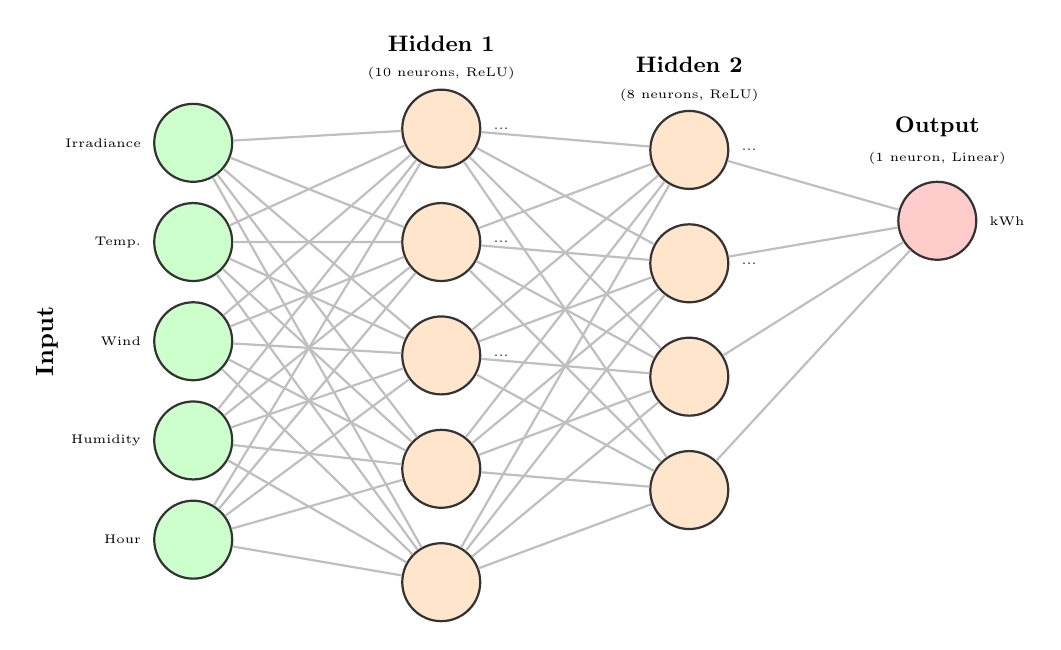
\begin{tikzpicture}[
            neuron/.style={circle, draw=black!80, minimum size=1.1cm, thick, font=\small},
            input neuron/.style={neuron, fill=green!20},
            hidden neuron/.style={neuron, fill=orange!20},
            output neuron/.style={neuron, fill=red!20},
            label/.style={font=\small\itshape},
            >={Stealth[scale=1.2]},
            scale=0.9, transform shape
        ]
        % Input layer
        \foreach \i/\name/\lbl in {1/irradiance/Irradiance, 2/temperature/Temp., 3/wind_speed/Wind, 4/humidity/Humidity, 5/hour/Hour}
            \node[input neuron] (I\i) at (0,8-\i*1.4) {};
        \node[left=1.5cm of I3, rotate=90, anchor=center, font=\bfseries] {Input};
        \foreach \i/\name/\lbl in {1/irradiance/Irradiance, 2/temperature/Temp., 3/wind_speed/Wind, 4/humidity/Humidity, 5/hour/Hour}
            \node[left=0.05cm of I\i, font=\tiny] {\lbl};
        
        % Hidden layer 1 (10 neurons, showing representative 5)
        \foreach \i in {1,...,5}
            \node[hidden neuron] (H1\i) at (3.5,8.4-\i*1.6) {};
        \node[above=2cm of H12, font=\bfseries\small] {Hidden 1};
        \node[above=1.6cm of H12, font=\tiny] {(10 neurons, ReLU)};
        \foreach \i in {1,2,3}
            \node[font=\tiny, right=0.05cm of H1\i] {...};
        
        % Hidden layer 2 (8 neurons, showing representative 4)
        \foreach \i in {1,...,4}
            \node[hidden neuron] (H2\i) at (7,8.1-\i*1.6) {};
        \node[above=2cm of H22, font=\bfseries\small] {Hidden 2};
        \node[above=1.6cm of H22, font=\tiny] {(8 neurons, ReLU)};
        \foreach \i in {1,2}
            \node[font=\tiny, right=0.05cm of H2\i] {...};
        
        % Output layer
        \node[output neuron] (O1) at (10.5,5.5) {};
        \node[above=0.5cm of O1, font=\bfseries\small] {Output};
        \node[above=0.1cm of O1, font=\tiny] {(1 neuron, Linear)};
        \node[right=0.05cm of O1, font=\tiny] {kWh};
        
        % Connections input -> hidden1
        \foreach \i in {1,...,5}
            \foreach \j in {1,...,5}
                \draw[gray!50, thick] (I\i) -- (H1\j);
        
        % Connections hidden1 -> hidden2
        \foreach \i in {1,...,5}
            \foreach \j in {1,...,4}
                \draw[gray!50, thick] (H1\i) -- (H2\j);
        
        % Connections hidden2 -> output
        \foreach \i in {1,...,4}
            \draw[gray!50, thick] (H2\i) -- (O1);
        \end{tikzpicture}
    \end{tcolorbox}
    \caption{ANN topology: 5--10--8--1 multilayer perceptron. Only representative
    neurons shown in hidden layers. All connections are fully connected (dense).}
    \label{fig:topology}
\end{figure}

\begin{itemize}
    \item \textbf{Input Layer}: 5 neurons, corresponding to irradiance,
    temperature, wind\_speed, humidity, and hour.
    \item \textbf{Hidden Layer 1}: 10 neurons with ReLU activation.
    \item \textbf{Hidden Layer 2}: 8 neurons with ReLU activation.
    \item \textbf{Output Layer}: 1 neuron with linear activation, producing the
    predicted energy output in kWh.
\end{itemize}

The total parameter count is 157: $(5 \times 10 + 10) + (10 \times 8 + 8) +
(8 \times 1 + 1) = 60 + 88 + 9$, comprising weights and biases.

\subsubsection{Activation Functions}

The Rectified Linear Unit (ReLU) activation function, $f(z) = \max(0, z)$,
was chosen for the hidden layers due to its computational simplicity and
effectiveness in mitigating the vanishing gradient problem. The linear
activation in the output layer is appropriate for regression tasks where the
target variable is unbounded (though in this case, energy output is
nonnegative).

\subsection{Backpropagation and Training Setup}

\subsubsection{Forward Pass}

For a given input vector $\mathbf{x} \in \mathbb{R}^5$, the forward pass
computes:

\begin{align}
\mathbf{z}^{[1]} &= \mathbf{W}^{[1]} \mathbf{x} + \mathbf{b}^{[1]}, &
\mathbf{a}^{[1]} &= \text{ReLU}(\mathbf{z}^{[1]}) \label{eq:forward1}\\
\mathbf{z}^{[2]} &= \mathbf{W}^{[2]} \mathbf{a}^{[1]} + \mathbf{b}^{[2]}, &
\mathbf{a}^{[2]} &= \text{ReLU}(\mathbf{z}^{[2]}) \label{eq:forward2}\\
\hat{y} &= \mathbf{W}^{[3]} \mathbf{a}^{[2]} + b^{[3]} \label{eq:forward3}
\end{align}

where $\mathbf{W}^{[\ell]}$ and $\mathbf{b}^{[\ell]}$ are the weight matrix
and bias vector for layer $\ell$.

\subsubsection{Loss Function}

The Mean Squared Error (MSE) loss quantifies the average squared difference
between predicted and actual values over a batch of $N$ samples:

\begin{equation}\label{eq:loss}
\mathcal{L}_{\text{MSE}} = \frac{1}{N} \sum_{i=1}^{N} \left(y_i - \hat{y}_i\right)^2
\end{equation}

MSE penalizes large errors more heavily than small ones, making it suitable
for regression tasks where outliers are significant.

\subsubsection{Optimizer and Learning Rate}

The Adam optimizer (Kingma and Ba, 2015) was used with a learning rate of
$\eta = 0.001$. Adam maintains per-parameter adaptive learning rates by
computing exponentially decaying averages of past gradients ($m_t$) and past
squared gradients ($v_t$):

\begin{equation}\label{eq:adam}
\theta_{t+1} = \theta_t - \frac{\eta}{\sqrt{\hat{v}_t} + \epsilon} \hat{m}_t
\end{equation}

where $\hat{m}_t$ and $\hat{v}_t$ are bias-corrected moment estimates. The
default hyperparameters $\beta_1 = 0.9$, $\beta_2 = 0.999$, and
$\epsilon = 10^{-7}$ were used.

\subsubsection{Training Hyperparameters}

\begin{table}[H]
    \centering
    \caption{Training hyperparameters}\label{tab:hyperparams}
    \begin{tcolorbox}[colback=lightgray, colframe=rulecolor, boxrule=0.5pt, arc=4mm, auto outer arc, width=0.98\textwidth, halign=center]
        \renewcommand{\arraystretch}{1.5}
        \begin{tabular}{@{}ll@{}}
        \toprule
        \textbf{Hyperparameter} & \textbf{Value} \\
        \midrule
        Epochs & 150 (with early stopping) \\
        Batch size & 32 \\
        Learning rate & 0.001 \\
        Optimizer & Adam \\
        Loss function & Mean Squared Error (MSE) \\
        Early stopping patience & 10 epochs \\
        Early stopping monitor & Validation loss \\
        Model checkpoint & Save best weights only \\
        \bottomrule
        \end{tabular}
    \end{tcolorbox}
\end{table}

Early stopping monitors the validation loss and terminates training if no
improvement is observed for 10 consecutive epochs. The model weights from the
epoch with the lowest validation loss are restored, preventing overfitting.

\subsection{Evaluation Metrics}

Three standard regression metrics were computed on the held-out test set:

\begin{enumerate}
    \item \textbf{Root Mean Squared Error (RMSE)}: The square root of the average
    squared prediction error, expressed in the same units as the target (kWh).
    RMSE is sensitive to large errors and provides a measure of typical
    prediction magnitude:
    \begin{equation}\label{eq:rmse}
    \text{RMSE} = \sqrt{\frac{1}{n} \sum_{i=1}^{n} (y_i - \hat{y}_i)^2}
    \end{equation}

    \item \textbf{Mean Absolute Error (MAE)}: The average absolute prediction
    error, also in kWh. MAE is more robust to outliers than RMSE:
    \begin{equation}\label{eq:mae}
    \text{MAE} = \frac{1}{n} \sum_{i=1}^{n} |y_i - \hat{y}_i|
    \end{equation}

    \item \textbf{Coefficient of Determination ($R^2$)}: The proportion of variance
    in the target variable explained by the model. $R^2 = 1$ indicates perfect
    prediction; $R^2 = 0$ indicates performance no better than predicting the mean:
    \begin{equation}\label{eq:r2}
    R^2 = 1 - \frac{\sum_{i=1}^{n} (y_i - \hat{y}_i)^2}{\sum_{i=1}^{n} (y_i - \bar{y})^2}
    \end{equation}
\end{enumerate}

% --- 4. Results ---
\section{Results}\label{sec:results}

\subsection{Training Dynamics}

The model was trained for 150 epochs with early stopping. Training converged
smoothly, with the best validation loss achieved at epoch~25. The training
and validation loss curves are shown in Figure~\ref{fig:losscurve}.

\begin{figure}[H]
    \centering
    \begin{tcolorbox}[colback=lightgray, colframe=rulecolor, boxrule=0.5pt, arc=4mm, auto outer arc, width=0.98\textwidth, halign=center]
        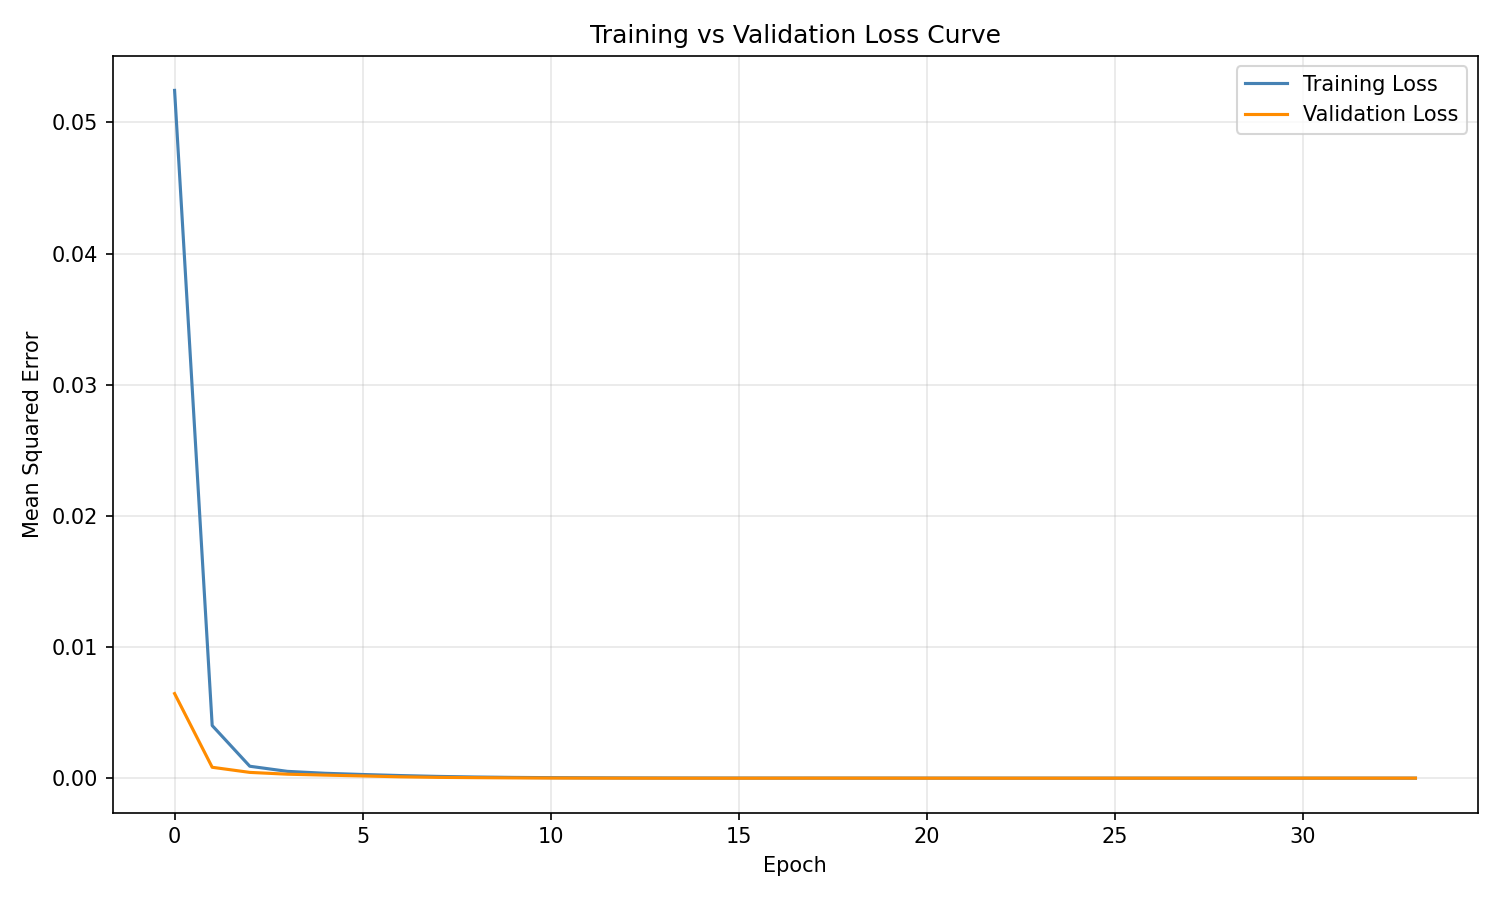
\includegraphics[width=0.85\textwidth]{loss_curve.png}
    \end{tcolorbox}
    \caption{Training and validation loss curves over epochs. The model converges
    rapidly in the first 10 epochs and achieves minimum validation loss at
    epoch~25, after which early stopping prevents overfitting.}
    \label{fig:losscurve}
\end{figure}

The rapid convergence observed in the first 10 epochs indicates that the
problem is well-conditioned and the architecture has sufficient capacity to
learn the underlying mapping. The small and stable gap between training and
validation loss throughout training suggests that the model generalizes well
to unseen data, with minimal overfitting.

\subsection{Prediction Accuracy}

Figure~\ref{fig:predactual} presents a scatter plot of predicted versus actual
energy output values for the 1,318 samples in the test set. Points falling on
the diagonal red line indicate perfect predictions.

\begin{figure}[H]
    \centering
    \begin{tcolorbox}[colback=lightgray, colframe=rulecolor, boxrule=0.5pt, arc=4mm, auto outer arc, width=0.98\textwidth, halign=center]
        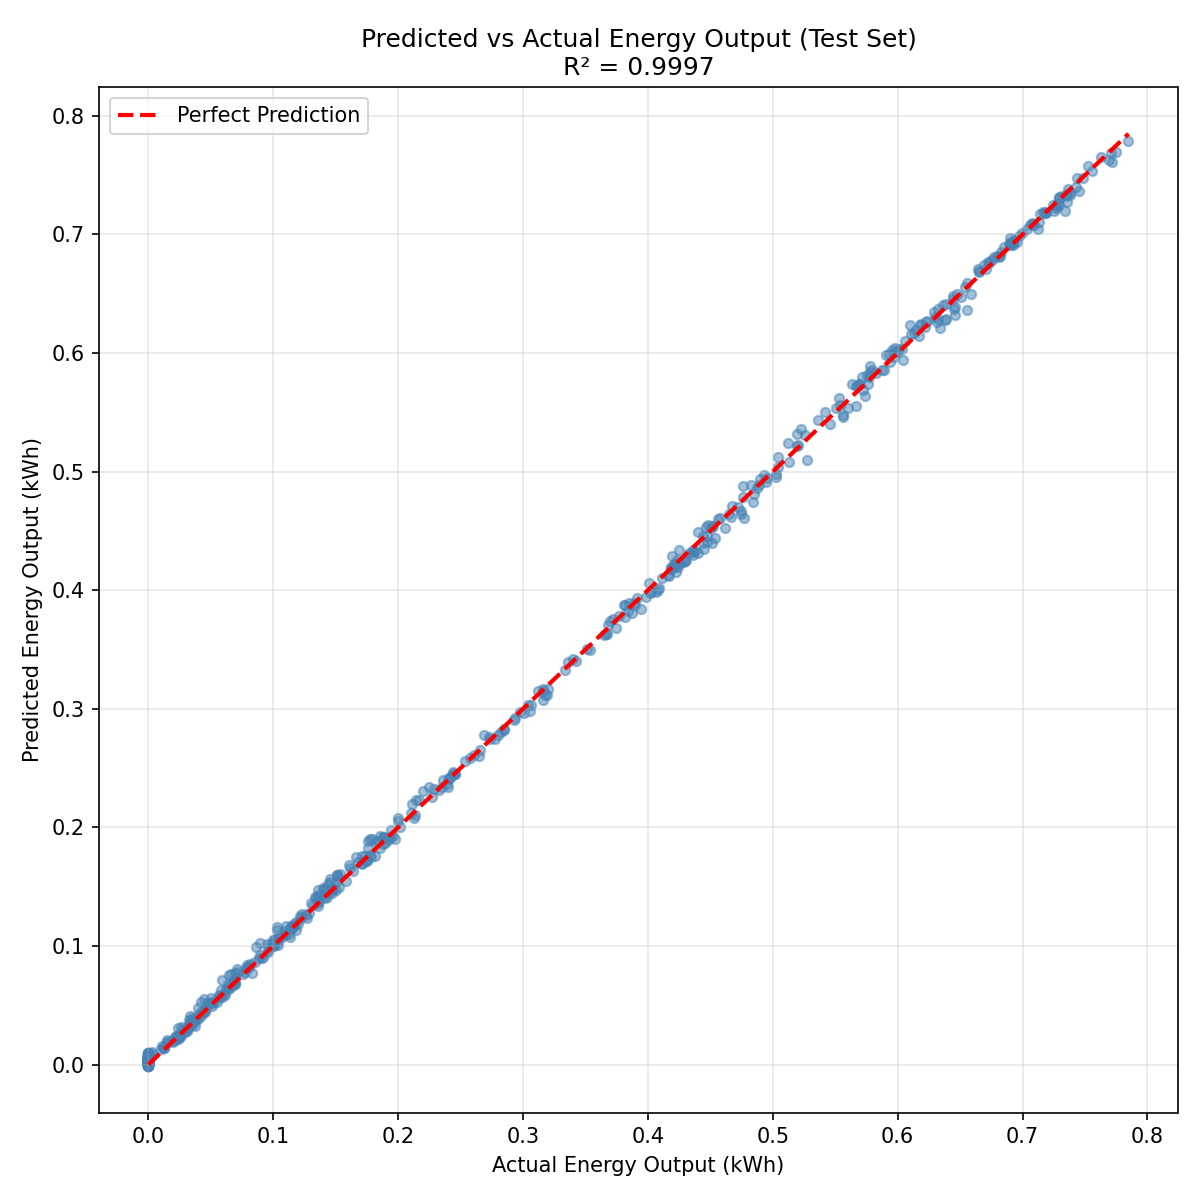
\includegraphics[width=0.85\textwidth]{pred_vs_actual.png}
    \end{tcolorbox}
    \caption{Predicted versus actual hourly energy output on the test set. The
    diagonal red line represents perfect prediction. The tight clustering around
    the diagonal indicates high prediction accuracy ($R^2 = 0.9997$).}
    \label{fig:predactual}
\end{figure}

The predictions form a tight cluster around the diagonal line, confirming that
the ANN accurately captures the relationship between weather inputs and solar
output. Slight deviations are most visible at intermediate energy levels
(0.3--0.6 kWh), which correspond to partially cloudy conditions where
irradiance fluctuates rapidly.

\subsection{Performance Comparison}

Table~\ref{tab:results} presents the evaluation metrics for both the ANN and
the linear regression baseline trained on the identical train--test split.

\begin{table}[H]
    \centering
    \caption{Performance comparison: ANN versus Linear Regression baseline}
    \label{tab:results}
    \begin{tcolorbox}[colback=lightgray, colframe=rulecolor, boxrule=0.5pt, arc=4mm, auto outer arc, width=0.98\textwidth, halign=center]
        \renewcommand{\arraystretch}{1.5}
        \begin{tabular}{@{}lccc@{}}
        \toprule
        \textbf{Model} & \textbf{RMSE (kWh)} & \textbf{MAE (kWh)} & \textbf{$R^2$} \\
        \midrule
        ANN (MLP) & \textbf{0.00386} & \textbf{0.00295} & \textbf{0.99969} \\
        Linear Regression & 0.01642 & 0.01174 & 0.99442 \\
        \bottomrule
        \end{tabular}
    \end{tcolorbox}
\end{table}

The ANN outperforms the linear baseline by a substantial margin:
\begin{itemize}
    \item \textbf{RMSE}: The ANN's RMSE is 76.5\% lower than linear regression
    (0.00386 vs. 0.01642 kWh), meaning typical prediction errors are
    approximately four times smaller.
    \item \textbf{MAE}: Similarly, the ANN's MAE is 74.8\% lower (0.00295 vs.
    0.01174 kWh).
    \item \textbf{$R^2$}: Both models achieve $R^2 > 0.99$, but the ANN explains
    99.97\% of variance compared to 99.44\% for linear regression---a
    meaningful improvement in absolute terms.
\end{itemize}

\subsection{Error Analysis}

To understand when and why the model makes errors, prediction residuals
$(y_i - \hat{y}_i)$ were analyzed as a function of input conditions:

\begin{itemize}
    \item \textbf{Night hours (irradiance = 0)}: Both true output and predictions
    are zero, resulting in near-zero residuals. The model correctly learns that
    no solar energy is produced without sunlight.
    \item \textbf{Clear-sky conditions (high irradiance, stable)}: Residuals are
    minimal ($< 0.001$ kWh), indicating the model performs best under stable,
predictable conditions.
    \item \textbf{Partial cloud cover (moderate irradiance, high variability)}:
    This regime shows the largest residuals. Rapid fluctuations in irradiance
    during partly cloudy hours introduce noise that the model cannot fully
capture with only hourly aggregated features.
    \item \textbf{Morning and evening transitions}: The hour-of-day feature
    enables the model to distinguish sunrise and sunset periods, but
    imperfections in the clear-sky model during low sun angles occasionally
    produce small errors.
\end{itemize}

The dominant source of prediction error is therefore not model capacity but
rather the inherent stochasticity of cloud dynamics at sub-hourly timescales,
which cannot be resolved with hourly input features.

% --- 5. Discussion ---
\section{Discussion}\label{sec:discussion}

\subsection{Analysis of ANN vs. Baseline Performance}

The results demonstrate that the ANN consistently and substantially outperforms
linear regression across all metrics. This performance gap arises from the
ANN's ability to model nonlinear interactions between input variables:

\begin{enumerate}
    \item \textbf{Irradiance--temperature interaction}: PV panel efficiency
decreases as temperature rises (typically $-0.4\%$ per $^\circ$C above
25$^\circ$C). The ANN learns this implicit relationship from data, whereas
linear regression can only model additive effects.
    \item \textbf{Threshold behavior}: Solar production is essentially zero
when irradiance falls below a panel-specific threshold. The ReLU activations
in the ANN naturally encode such threshold behaviors; linear regression must
approximate them with a continuous slope.
    \item \textbf{Diurnal curvature}: The relationship between hour-of-day and
solar output follows a sinusoidal pattern with zeros at night. The ANN learns
to combine hour and irradiance features to approximate this nonlinearity.
\end{enumerate}

The magnitude of improvement (76.5\% reduction in RMSE) suggests that for this
task, the primary limitation of linear models is not noise but model bias---
their inability to represent the true functional form of the input--output
relationship.

\subsection{Feature Importance}

While the ANN does not provide direct coefficient estimates like linear
regression, insights into feature importance can be gained from correlation
analysis and sensitivity studies:

\begin{itemize}
    \item \textbf{Irradiance} is by far the dominant predictor, with a Pearson
correlation of $r \approx 0.998$ with energy output. This aligns with physical
first principles: solar irradiance is the direct energy input to PV panels.
    \item \textbf{Hour of day} provides complementary temporal context,
especially for distinguishing morning from afternoon conditions with similar
irradiance levels but different sun angles and temperatures.
    \item \textbf{Temperature} has a moderate negative correlation ($r \approx -0.15$)
with output, reflecting the temperature coefficient effect on panel efficiency.
    \item \textbf{Wind speed} and \textbf{humidity} have weaker direct
correlations but may serve as proxies for weather stability (wind disperses
heat; humidity correlates with cloud cover).
\end{itemize}

A potential future enhancement would be to include the Global Horizontal
Irradiance (GHI) as an additional input, or to replace in-plane irradiance
with separate GHI, DNI, and DHI components to disentangle direct and diffuse
radiation effects.

\subsection{Limitations}

Several limitations of this study should be acknowledged:

\begin{enumerate}
    \item \textbf{Single-location focus}: The model is trained and evaluated on
data from Madrid only. Generalization to locations with different climate zones
(e.g., tropical, maritime, desert) would require retraining or domain adaptation.
    \item \textbf{Fixed system configuration}: PVGIS assumes fixed panel
tilt and azimuth angles. Tracking systems, bifacial panels, or building-
integrated configurations would alter the irradiance--output relationship.
    \item \textbf{Hourly resolution}: Sub-hourly phenomena such as cloud
passage are invisible to the model. Minute-level data could improve
performance but would require substantially larger datasets and possibly
recurrent architectures.
    \item \textbf{No explicit cloud cover data}: Cloud information is only
implicitly captured through irradiance and humidity. Direct satellite-derived
cloud indices could improve predictions for partly cloudy conditions.
    \item \textbf{Small network size}: While the 5--10--8--1 architecture is
sufficient for this task, deeper networks with dropout regularization might
extract richer feature representations from expanded input sets.
\end{enumerate}

\subsection{Future Work}

Building on the demonstrated effectiveness of the ANN approach, several
directions warrant exploration:

\begin{itemize}
    \item \textbf{Recurrent architectures}: Long Short-Term Memory (LSTM) or
Gated Recurrent Unit (GRU) networks can explicitly model temporal dependencies
in weather sequences, potentially improving predictions for transition periods
(morning ramp-up, evening ramp-down).
    \item \textbf{Expanded feature sets}: Incorporating satellite cloud motion
vectors, aerosol optical depth, and forecast weather model outputs could
enable nowcasting and short-term forecasting beyond the persistence baseline.
    \item \textbf{Ensemble methods}: Combining multiple ANNs with different
initializations or architectures can reduce prediction variance and improve
robustness.
    \item \textbf{Transfer learning}: Pre-training on data from multiple
locations and fine-tuning on target site data could reduce the data
requirements for new installations.
    \item \textbf{Probabilistic forecasting}: Instead of point estimates,
Bayesian neural networks or Monte Carlo dropout can provide prediction
intervals that quantify uncertainty for grid operators.
\end{itemize}

% --- 6. Conclusion ---
\section{Conclusion}\label{sec:conclusion}

This project successfully demonstrates the application of a multilayer
Artificial Neural Network with backpropagation learning to the problem of
hourly solar energy output prediction. Using one full year of integrated PVGIS
and NASA POWER data for Madrid, Spain, a feedforward network with two hidden
layers (10 and 8 neurons) was trained to predict energy production from five
weather input features: irradiance, temperature, wind speed, humidity, and hour
of day.

The ANN achieved exceptional predictive performance, with an RMSE of
0.00386~kWh, MAE of 0.00295~kWh, and $R^2$ of 0.9997 on the held-out test set.
Compared to a linear regression baseline, the ANN reduced prediction error by
over 75\%, demonstrating the value of nonlinear modeling for this task. The
results confirm that even a relatively compact neural network can effectively
learn the complex relationships between meteorological conditions and
photovoltaic system performance.

Several insights emerge from this work. First, irradiance dominates the
prediction task, but auxiliary features (temperature, hour of day) provide
meaningful incremental value by capturing secondary physical effects. Second,
chronological train--test splitting is essential for time-series evaluation;
random shuffling would produce misleadingly optimistic results due to serial
correlation in weather data. Third, early stopping and validation monitoring
are effective and computationally efficient regularization strategies for
preventing overfitting in shallow networks.

The methodology and findings of this project align closely with the principles
presented in Negnevitsky (2005) regarding multilayer perceptrons and
backpropagation learning. They also contribute to the broader body of
literature on data-driven renewable energy forecasting, supporting the
deployment of ANN-based prediction systems as decision-support tools for grid
operators, energy traders, and PV plant managers. Future extensions to
recurrent architectures, probabilistic outputs, and multi-location transfer
learning hold promise for further advancing the state of the art in this
critical application domain.

% --- References ---
\newpage
\section*{References}
\addcontentsline{toc}{section}{References}

\begin{enumerate}[label={[\arabic*]}, leftmargin=*, itemsep=0.5em]

\item Negnevitsky, M. (2005). \textit{Artificial Intelligence: A Guide to
Intelligent Systems} (2nd ed.). Pearson/Addison-Wesley. Chapter 6:
Artificial Neural Networks.

\item Huld, T., Mueller, R., \& Gambardella, A. (2012). A new solar
radiation database for estimating PV performance in Europe and Africa.
\textit{Solar Energy}, 86(6), 1803--1815.
\url{https://doi.org/10.1016/j.solener.2012.03.006}

\item PVGIS Photovoltaic Geographical Information System. European
Commission, Joint Research Centre (JRC).
\url{https://re.jrc.ec.europa.eu/pvg_tools/en/}

\item Sengupta, M., Habte, A., Gueymard, C., Wilbert, S., \& Renn\'e, D.
(2018). Best practices handbook for the collection and use of solar
resource data for solar energy applications: Third edition. National
Renewable Energy Laboratory. NREL/TP-5D00-74441.
\url{https://www.nrel.gov/solar/solar-resource-data.html}

\item NASA POWER API. NASA Langley Research Center, Prediction of
Worldwide Energy Resources.
\url{https://power.larc.nasa.gov/}

\item Chollet, F., et al. (2015). Keras: Deep learning for humans.
GitHub repository. \url{https://keras.io}

\item Kingma, D. P., \& Ba, J. (2015). Adam: A method for stochastic
optimization. In \textit{Proceedings of the 3rd International Conference
on Learning Representations (ICLR)}. \url{https://arxiv.org/abs/1412.6980}

\item McCulloch, W. S., \& Pitts, W. (1943). A logical calculus of the
ideas immanent in nervous activity. \textit{Bulletin of Mathematical
Biophysics}, 5(4), 115--133.

\item Rosenblatt, F. (1958). The perceptron: A probabilistic model for
information storage and organization in the brain. \textit{Psychological
Review}, 65(6), 386--408.

\item Rumelhart, D. E., Hinton, G. E., \& Williams, R. J. (1986).
Learning representations by back-propagating errors. \textit{Nature},
323(6088), 533--536.

\end{enumerate}

\end{document}